\chapter{Literature Review}
\label{ch:lit}

\section{Approach}

This chapter keeps the fifteen studies reviewed in the Phase 2 report and adds the work that Phase 3
depends on: external validation, shortcut learning and input-blind baselines, calibration and
abstention, and vision-language models. Every citation resolves to an entry of the project
bibliography that was checked against Crossref, OpenAlex, Semantic Scholar and arXiv in November
2026. Every number attributed to a study below was checked against that study's published abstract;
where a Phase 2 statement could not be confirmed it was removed or rewritten, and the correction is
noted. Two Phase 2 entries had been attached to the wrong reference (Sections~\ref{lit:albano}
and~\ref{lit:iacob}); both now cite the paper they describe.

\section{Reviewed Studies}

\subsection{Detection of Dental Caries Under Fixed Dental Prostheses~\cite{ayhan2025detection}}
\litmeta{Ayhan et al.}{2025}{BMC Oral Health}
% {C101}
\litpart{Problem addressed.} Caries beneath fixed dental prostheses is hard to see on panoramic
radiographs because the restoration obscures the tooth underneath.
\litpart{Method used.} Panoramic radiographs of 1,004 patients were split 90/10 for training and
test. A YOLOv7 model first finds and crops the regions containing prostheses; on 2,467 such crops a
second stage detects caries with YOLOv7 and with YOLOv7 extended by a convolutional block attention
module (CBAM) (Figure~\ref{fig:lit-ayhan}).

\begin{figure}[!htbp]
\centering
\optionalgraphics[width=0.62\textwidth]{figures/phase2/p2_2_01_yolov7_cbam.jpg}
\caption[YOLOv7 + CBAM architecture for caries detection]{YOLOv7 + CBAM architecture for caries
detection under prostheses (figure reproduced from~\cite{ayhan2025detection}, as in the Phase 2
report).}
\label{fig:lit-ayhan}
\end{figure}

\litpart{Strengths.}
\begin{itemize}
\item The attention model reached recall 0.827, precision 0.834, mAP 0.846 and F1 0.830 on the
  caries-under-prosthesis task.
\item The two-stage design narrows the search to the prosthesis region before looking for caries.
\end{itemize}
\litpart{Limitations.}
\begin{itemize}
\item Only an internal 90/10 split is reported; no external cohort.
\item Caries only, with no numbering, severity grading or periodontal analysis.
\end{itemize}

\subsection{AI-Powered Dental Caries Detection from Intraoral Images~\cite{khuwaja2024ai}}
\litmeta{Khuwaja et al.}{2024}{IEEE INMIC}
% {C102}
\litpart{Problem addressed.} Early caries detection from smartphone photographs of the mouth, to make
screening cheaper and more accessible in low- and middle-income areas.
\litpart{Method used.} YOLO, EfficientDet, MobileNet and ResNet-50 detectors are compared on
smartphone intraoral images; YOLOv8 and ResNet-50 are built into a mobile application
(Figure~\ref{fig:lit-khuwaja}).

\begin{figure}[!htbp]
\centering
\optionalgraphics[width=0.52\textwidth]{figures/phase2/p2_2_02_intraoral_pipeline.jpg}
\caption[Mobile application workflow for intraoral caries screening]{Mobile application workflow for
intraoral caries screening (figure reproduced from~\cite{khuwaja2024ai}, as in the Phase 2 report).}
\label{fig:lit-khuwaja}
\end{figure}

\litpart{Strengths.}
\begin{itemize}
\item Targets accessibility: screening on a phone, without radiographic equipment.
\item Compares several detector families; the abstract reports ResNet-50 as the most effective and
  MobileNet as a strong alternative.
\end{itemize}
\litpart{Limitations.}
\begin{itemize}
\item Photographs show only visible tooth surfaces, with no radiographic depth.
\item The abstract reports no quantitative metric, so the result cannot be compared with
  radiograph-based systems. \emph{(The Phase 2 report quoted a dataset size and mAP that the abstract
  does not contain; both are omitted here.)}
\end{itemize}

\subsection{Advanced AI-Assisted Panoramic Radiograph Analysis for Periodontal Prognostication~\cite{jundaeng2025advanced}}
\litmeta{Jundaeng et al.}{2025}{Frontiers in Dental Medicine}
% {C103}
\litpart{Problem addressed.} Radiographic assessment of alveolar bone loss is subjective and
labour-intensive; the study automates it and adds a per-tooth periodontal prognosis.
\litpart{Method used.} Two thousand panoramic radiographs from one device were enhanced, and YOLOv8
models segment the teeth, the cemento-enamel junction (CEJ) and the alveolar bone level, from which
bone loss is quantified and a prognosis is assigned to each tooth (Figure~\ref{fig:lit-jundaeng}).

\begin{figure}[!htbp]
\centering
\optionalgraphics[width=0.42\textwidth]{figures/phase2/p2_2_03_periodontal_dual_yolo.jpg}
\caption[YOLO-based pipeline for periodontal bone-loss assessment]{YOLO-based pipeline for
periodontal bone-loss assessment and prognosis (figure reproduced from~\cite{jundaeng2025advanced},
as in the Phase 2 report).}
\label{fig:lit-jundaeng}
\end{figure}

\litpart{Strengths.}
\begin{itemize}
\item Tooth segmentation reached 97\% accuracy (F1 0.80), and CEJ and bone-level segmentation 98\%
  accuracy with F1 0.90.
\item Produces tooth-level bone-loss estimates, which is what periodontal staging needs.
\end{itemize}
\litpart{Limitations.}
\begin{itemize}
\item All radiographs came from the same device, so variation in acquisition is not tested.
\item No caries analysis. \emph{(The Phase 2 report quoted an mAP of 0.995 that the abstract does not
  contain; it is omitted here.)}
\end{itemize}

\subsection{Detection of Cavities from Dental Panoramic X-ray Images Using Nested U-Net Models~\cite{alharbi2023detection}}
\litmeta{Alharbi et al.}{2023}{Applied Sciences}
% {C104}
\litpart{Problem addressed.} Pixel-level segmentation of carious cavities on panoramic radiographs.
\litpart{Method used.} U-Net, U-Net++ and U-Net3+ are trained on 1,500 panoramic radiographs; the
nested variants aggregate multi-scale features to sharpen the cavity boundary
(Figure~\ref{fig:lit-alharbi}).

\begin{figure}[!htbp]
\centering
\optionalgraphics[width=0.66\textwidth]{figures/phase2/p2_2_04_nested_unet.jpg}
\caption[Nested U-Net architecture for cavity segmentation]{Nested U-Net architecture for cavity
segmentation (figure reproduced from~\cite{alharbi2023detection}, as in the Phase 2 report).}
\label{fig:lit-alharbi}
\end{figure}

\litpart{Strengths.}
\begin{itemize}
\item U-Net3+ reached 95\% testing accuracy, the best of the three variants.
\item Segmentation gives a precise outline of each lesion for visual interpretation.
\end{itemize}
\litpart{Limitations.}
\begin{itemize}
\item Pixel accuracy is dominated by healthy background and is not a lesion- or tooth-level measure.
\item No tooth numbering, severity grade or multi-disease output.
\end{itemize}

\subsection{Deep Learning-Based Recognition of Periodontitis and Dental Caries in Dental X-ray Images~\cite{chen2023deep}}
\litmeta{Chen et al.}{2023}{Bioengineering}
% {C105}
\litpart{Problem addressed.} Recognising both periodontitis and caries on the same radiographs.
\litpart{Method used.} A two-stage pipeline: YOLOv7 detects teeth on periapical radiographs, and an
EfficientNet-B0 classifier labels each cropped tooth (Figure~\ref{fig:lit-chen23}).

\begin{figure}[!htbp]
\centering
\optionalgraphics[width=0.72\textwidth]{figures/phase2/p2_2_05_two_stage_pipeline.jpg}
\caption[Two-stage detection and classification pipeline]{Two-stage pipeline combining tooth
detection and classification (figure reproduced from~\cite{chen2023deep}, as in the Phase 2 report).}
\label{fig:lit-chen23}
\end{figure}

\litpart{Strengths.}
\begin{itemize}
\item Two diseases in one system; for periodontitis the area under the receiver operating characteristic (ROC) curve was 98.67\% and the
  area under the precision--recall curve 98.38\%.
\item The detect-then-classify structure is the same tooth-centric decomposition this project uses.
\end{itemize}
\litpart{Limitations.}
\begin{itemize}
\item Periapical radiographs only, not panoramic.
\item No severity grade and no explanation of individual predictions.
\end{itemize}

\subsection{YOLO-Based Panoramic Dental X-ray Image Analysis~\cite{nassiri2025yolo}}
\litmeta{Nassiri and Akhloufi}{2025}{Neural Computing and Applications}
% {C106}
\litpart{Problem addressed.} Automated analysis of panoramic dental X-rays with YOLO-family detectors.
\litpart{Method used.} A multi-step pipeline of YOLO models for detecting teeth and dental conditions
on panoramic X-rays (Figure~\ref{fig:lit-nassiri}).

\begin{figure}[!htbp]
\centering
\optionalgraphics[width=0.66\textwidth]{figures/phase2/p2_2_06_yolo_panoramic.jpg}
\caption[YOLO-based framework for panoramic dental X-ray analysis]{YOLO-based framework for panoramic
dental X-ray analysis (figure reproduced from~\cite{nassiri2025yolo}, as in the Phase 2 report).}
\label{fig:lit-nassiri}
\end{figure}

\litpart{Strengths.}
\begin{itemize}
\item One-stage YOLO detectors give fast inference, which suits screening.
\item Provides a baseline design for tooth-level localisation on panoramic images.
\end{itemize}
\litpart{Limitations.}
\begin{itemize}
\item No abstract of this article is indexed by Crossref, OpenAlex or Semantic Scholar, so its
  reported figures could not be checked for this report. \emph{(The Phase 2 report quoted a
  comparison of YOLO versions on DENTEX with an mAP50 near 0.978; it is not relied on here.)}
\end{itemize}

\subsection{Deep Learning for Automatic Tooth Caries Segmentation in Paediatric Radiographs~\cite{asci2024deep}}
\litmeta{Asci et al.}{2024}{Children (MDPI)}
% {C107}
\litpart{Problem addressed.} Caries segmentation on panoramic radiographs of children, where primary,
mixed and permanent dentition differ.
\litpart{Method used.} A U-Net trained on 6,075 paediatric panoramic radiographs segments carious
regions; results are reported for each dentition group and in total (Figure~\ref{fig:lit-asci}).

\begin{figure}[!htbp]
\centering
\optionalgraphics[width=0.52\textwidth]{figures/phase2/p2_2_07_unet_pediatric.jpg}
\caption[U-Net segmentation for paediatric caries detection]{U-Net segmentation for paediatric caries
detection (figure reproduced from~\cite{asci2024deep}, as in the Phase 2 report).}
\label{fig:lit-asci}
\end{figure}

\litpart{Strengths.}
\begin{itemize}
\item Over all dentition groups: sensitivity 0.8269, precision 0.9123 and F1 0.8675.
\item Handles three dentition stages with one model.
\end{itemize}
\litpart{Limitations.}
\begin{itemize}
\item Caries only; no severity grade and no periodontal analysis.
\item Trained and evaluated on children only.
\end{itemize}

\subsection{CariesXrays: Enhancing Caries Detection via Feature Pyramid Contrastive Learning~\cite{chen2024cariesxrays}}
\litmeta{Chen et al.}{2024}{AAAI Conference on Artificial Intelligence}
% {C108}
\litpart{Problem addressed.} Subtle caries lesions are hard to detect in hospital-scale panoramic
datasets.
\litpart{Method used.} The authors release CariesXrays, 6,000 panoramic radiographs with 13,783
annotated caries instances, and propose feature pyramid contrastive learning (FPCL) to sharpen lesion
features in a detector.
\litpart{Strengths.}
\begin{itemize}
\item A large public benchmark with lesion-level boxes; FPCL reports AP50 84.1.
\item This project's lesion detector trains on CariesXrays and is compared with FPCL on it
  (Section~\ref{sec:res-train}).
\end{itemize}
\litpart{Limitations.}
\begin{itemize}
\item Lesion boxes without tooth identity, so it cannot by itself produce a tooth-indexed report.
\item No severity grade. \emph{(The Phase 2 report showed the Asci et al.\ figure for this entry by
  mistake; it is not repeated.)}
\end{itemize}

\subsection{AI-Dentify: Deep Learning for Proximal Caries Detection on Bitewing X-rays~\cite{perez2024ai}}
\litmeta{Pérez de Frutos et al.}{2024}{BMC Oral Health}
% {C109}
\litpart{Problem addressed.} Proximal caries between teeth on bitewing radiographs, where surfaces
overlap.
\litpart{Method used.} YOLOv5, RetinaNet and EfficientDet are trained on 13,887 bitewings from the
HUNT4 Oral Health Study and compared with dental clinicians (Figure~\ref{fig:lit-aidentify}).

\begin{figure}[!htbp]
\centering
\optionalgraphics[width=0.6\textwidth]{figures/phase2/p2_2_09_ai_dentify.jpg}
\caption[Detection of proximal caries in bitewing X-rays]{Detection of proximal caries in bitewing
X-rays (figure reproduced from~\cite{perez2024ai}, as in the Phase 2 report).}
\label{fig:lit-aidentify}
\end{figure}

\litpart{Strengths.}
\begin{itemize}
\item A large population-study dataset and a comparison with clinicians; YOLOv5 reported 0.647 mean
  average precision and 0.548 mean F1.
\end{itemize}
\litpart{Limitations.}
\begin{itemize}
\item Bitewing modality only; no periodontal analysis and no severity grade.
\end{itemize}

\subsection{Artificial Intelligence for Radiographic Detection of Caries Lesions: A Systematic Review~\cite{albano2024artificial}}
\label{lit:albano}
\litmeta{Albano et al.}{2024}{BMC Oral Health}
% {C110}
\litpart{Problem addressed.} How well AI models detect caries lesions on radiographs.
\litpart{Method used.} A systematic review of 20 studies (five periapical, nine bitewing and six
panoramic), assessed with QUADAS-2.
\litpart{Strengths.}
\begin{itemize}
\item Reports the spread of performance: sensitivity 0.44 to 0.86, specificity 0.85 to 0.98,
  accuracy 0.73 to 0.98 and area under the curve (AUC) 0.84 to 0.98.
\end{itemize}
\litpart{Limitations.}
\begin{itemize}
\item A review: no new experiment and no unified framework. \emph{(The Phase 2 report cited this entry
  as reference~[10], a different paper; it now cites the review itself.)}
\end{itemize}

\subsection{DenseNet201-Powered Dental Radiograph Classification~\cite{kaushik2025densenet201}}
\litmeta{Kaushik and Sharma}{2025}{IEEE ICPC2T}
% {C111}
\litpart{Problem addressed.} Multi-class classification of dental conditions on radiographs.
\litpart{Method used.} Transfer learning with DenseNet201 (ImageNet weights, Adam optimiser) on 29,815
dental X-ray images in five categories.
\litpart{Strengths.}
\begin{itemize}
\item Overall accuracy 91\%, with F1 0.95 for normal images and 0.91 for implants.
\end{itemize}
\litpart{Limitations.}
\begin{itemize}
\item Cavity detection was the weakest class, consistent with class imbalance.
\item Image-level labels give no lesion localisation and no tooth identity.
\end{itemize}

\subsection{Automated Detection of Periodontal Bone Loss in 2D Radiographs Using AI: A Systematic Review~\cite{iacob2025automated}}
\label{lit:iacob}
\litmeta{Iacob et al.}{2025}{Dentistry Journal (MDPI)}
% {C112}
\litpart{Problem addressed.} How effective AI architectures are at detecting periodontal bone loss on
periapical, bitewing and panoramic radiographs.
\litpart{Method used.} A PRISMA systematic review registered in PROSPERO, covering 20 diagnostic
accuracy studies published between 2019 and 2024, with risk of bias assessed by QUADAS-2.
\litpart{Strengths.}
\begin{itemize}
\item Brings the recent evidence together and identifies the main obstacle to comparison.
\end{itemize}
\litpart{Limitations.}
\begin{itemize}
\item The included studies use heterogeneous accuracy indices and imaging protocols, which limits
  comparison and reproducibility. \emph{(The Phase 2 report attached this entry to
  reference~[4]~\cite{muresanu2024automating}, a different study, and quoted an image count the
  review's abstract does not contain.)}
\end{itemize}

\subsection{The 2018 Classification of Periodontitis: Challenges from a Clinical Perspective~\cite{chmielewski20252018}}
\litmeta{Chmielewski et al.}{2025}{Dentistry Journal (MDPI)}
% {C113}
\litpart{Problem addressed.} The clinical difficulties of applying the 2018 AAP/EFP classification of
periodontitis.
\litpart{Method used.} A narrative review of studies on diagnostic accuracy and on inter- and
intra-examiner agreement when the classification is used, with and without implementation aids
(Figure~\ref{fig:lit-aapefp}).

\begin{figure}[!htbp]
\centering
\optionalgraphics[width=0.62\textwidth]{figures/phase2/p2_2_10_aap_efp_2018.jpg}
\caption[Clinical inputs to the 2018 AAP/EFP classification]{Clinical inputs to the 2018 AAP/EFP
classification of periodontitis (figure reproduced from~\cite{chmielewski20252018}, as in the Phase 2
report).}
\label{fig:lit-aapefp}
\end{figure}

\litpart{Strengths.}
\begin{itemize}
\item Shows why staging needs consistent, objective measurements.
\end{itemize}
\litpart{Limitations.}
\begin{itemize}
\item No AI implementation and no quantitative evaluation of an automated system.
\end{itemize}

\subsection{Automated Diagnosis of Dental Conditions in Panoramic X-rays with Ensemble Deep Learning~\cite{gamal2025automated}}
\litmeta{Gamal et al.}{2025}{IEEE IMSA}
% {C114}
\litpart{Problem addressed.} Interpreting panoramic radiographs for common pathologies (caries,
impacted teeth) and restorations (fillings, implants) more reliably than with one model.
\litpart{Method used.} CNNs with transfer learning, combined in an ensemble.
\litpart{Strengths.}
\begin{itemize}
\item More than 92\% classification accuracy; the ensemble improves stability.
\end{itemize}
\litpart{Limitations.}
\begin{itemize}
\item Higher computational cost than a single model; no lesion localisation or severity grade.
  \emph{(The Phase 2 report listed specific backbones, a crop count and a 92.93\% figure that the
  abstract does not contain; they are omitted here.)}
\end{itemize}

\subsection[AI-Driven Approaches for Enhancing Early Detection of Dental Caries]{AI-Driven Approaches for Enhancing Early Detection of\\ Dental Caries~\cite{sastika2025ai}}
\litmeta{Sastika and Marappan}{2025}{IEEE ICICKE}
% {C115}
\litpart{Problem addressed.} The state of AI for early caries detection.
\litpart{Method used.} A literature review of CNN classifiers, YOLO detectors, U-Net segmentation and
ensemble CNNs (Figure~\ref{fig:lit-sastika}).

\begin{figure}[!htbp]
\centering
\optionalgraphics[width=0.72\textwidth]{figures/phase2/p2_2_11_ai_caries_overview.jpg}
\caption[Overview of AI-driven approaches for early caries detection]{Overview of AI-driven approaches
for early caries detection (figure reproduced from~\cite{sastika2025ai}, as in the Phase 2 report).}
\label{fig:lit-sastika}
\end{figure}

\litpart{Strengths.}
\begin{itemize}
\item Summarises reported performance: accuracies of 85--99\%, precisions of 86--96\% and F1-scores
  of 87--94\%.
\end{itemize}
\litpart{Limitations.}
\begin{itemize}
\item A review: no experiment, no integration of several diseases and no treatment of deployment.
\end{itemize}

\section{Thematic Review}

\subsection{Datasets}

The project uses five public datasets. The Tufts Dental Database provides 1,000 OPGs with expert
tooth and abnormality annotations~\cite{panetta2022tufts}. DENTEX provides hierarchically annotated
quadrant, enumeration and diagnosis labels~\cite{hamamci2023dentex}. CariesXrays provides 6,000 OPGs
with lesion boxes~\cite{chen2024cariesxrays}. The multi-centre dataset of Li et al.\ was collected at
three hospitals in Ningxia and Shenzhen~\cite{li2024multicenter}. UFBA-425 provides 425 radiographs
with tooth annotations~\cite{budagam2024oralbbnet}. Combining public datasets is itself a research
topic: van Nistelrooij et al.\ merged OdontoAI tooth segmentations with DENTEX boxes and diagnoses to
predict segmentations, FDI numbers and diagnoses together~\cite{vannistelrooij2024combining}. % {C120}

\subsection{Detection, Numbering and Caries}

A systematic review of deep-learning caries detection found accuracies of 86.1--96.1\% on panoramic
radiographs, in studies whose quality and reporting it judged low~\cite{mohammadrahimi2022deep}.
Caries and periodontal analysis has used dual networks~\cite{lim2024dual}, dedicated convolutional
classifiers~\cite{bilal2024pdcnet}, U-Net variants~\cite{vickram2025extraction} and contrastive feature
pyramids~\cite{chen2024cariesxrays}. One study confirmed panoramic caries labels against bitewings
before training a YOLOv5 tooth detector and an Attention U-Net, on 500 radiographs with 1,792 caries
among 14,997 teeth~\cite{pornprasertsuk2025clinical}. Numbering is reported at very high figures:
class-averaged accuracy 0.9988 (F1 0.979) in one system~\cite{zancan2025ai}, and a multi-stage system
reports higher scores than earlier methods on Tufts and two other datasets~\cite{zhang2025reliable}. A meta-analysis
summarises deep-learning tooth detection and segmentation on OPGs~\cite{bonfanti2025deep}. Classifying
a tooth that is already cropped is easier than numbering under detector output, where teeth can be
missed or duplicated; this project reports numbering end to end (Section~\ref{sec:res-identity}). % {C121}

\subsection{Periodontal Bone Loss}

A systematic review and meta-analysis covers AI for alveolar bone loss and periodontitis on panoramic
and periapical radiographs~\cite{khubrani2025detection}. Published methods combine YOLOv8 tooth
detection with keypoint models for landmarks on periapical radiographs~\cite{wimalasiri2025ai},
super-resolution networks before segmentation on panoramic radiographs~\cite{kong2024integrating}, and
segmentation of the alveolar crest and CEJ on bitewings, evaluated by dental
professionals~\cite{lee2025evaluation}. A YOLOv8 model for several dental conditions was trained on
1,628 panoramic radiographs and validated externally on 180 from several
centres~\cite{muresanu2024automating}. The Phase 2 periodontal branch of this project, and its Phase 3
correction, are described in Sections~\ref{sec:sys-stage4} and~\ref{sec:res-stage4}. % {C122}

\subsection{Transfer and External Validation}

Of 516 medical-imaging AI studies published January--August 2018, only 31 (6\%) validated
externally~\cite{kim2019design}. Dental models tested elsewhere degrade: an apical-lesion model fell
from F1 54.1\% to 32.7\% at a second centre~\cite{krois2021generalizability}, and a YOLOv11 detector of
13 conditions fell from mAP@0.5 0.857 to 0.806 on external images, weakest on subtle pathology such as
caries~\cite{mutlu2026comparison}. One enumeration-then-caries detector held lesion sensitivity at
0.70 internally and 0.67 externally~\cite{bizjak2024advancing}. % {C123}

\subsection{Shortcuts and Input-Blind Baselines}

Shortcut learning predicts that a model will exploit any cue correlated with the
label~\cite{geirhos2020shortcut}, and other fields test for it with baselines that withhold the input
the task is about. Visual-question-answering models answered from language priors while ignoring the
image, inflating their apparent capability~\cite{goyal2017making}, and lost accuracy when answer
priors differed between training and test~\cite{agrawal2018dont}; in natural-language inference, a
model shown only the hypothesis, without the premise, scores above the majority class on many
datasets~\cite{poliak2018hypothesis}. In medical imaging, COVID-19 detectors relied on confounders
and failed at new hospitals~\cite{degrave2021ai}, and in a pneumonia task sorting radiographs by
hospital alone reached AUC 0.861 because prevalence differed between sites~\cite{zech2018variable}.
In the 49 task-relevant papers of the project's own survey of OPG analysis, none was noticed to
report an image-blind baseline (an observation, not a systematic count). % {C124} {C097}

\subsection{Calibration, Abstention and Vision-Language Models}

Temperature scaling~\cite{guo2017calibration} and isotonic regression~\cite{zadrozny2002isotonic} are
the calibration methods compared here, and abstention follows selective
classification~\cite{geifman2017selective}. Vision-language models (VLMs) are being adapted to dental
diagnosis~\cite{meng2026dentvlm}; this project uses Qwen2.5-VL~\cite{bai2025qwen25vl} as a general
comparator that needs no task training. % {C125}

\section{Comparative Analysis}

The comparison in Table~\ref{tab:lit-compare} places the studies that address panoramic analysis beside this project on
the capabilities a tooth-indexed report needs. A dash means the capability is not reported in the
study's abstract, which is not proof that the study lacks it.

\begin{table}[!htbp]
\centering
\caption[Capabilities of reviewed panoramic-radiograph systems]{Capabilities of reviewed
panoramic-radiograph systems against this project. \checkmark: reported in the abstract;
---: not reported there.}
\label{tab:lit-compare}
\small
\begin{tabular}{@{}L{3.9cm}C{1.35cm}C{1.35cm}C{1.2cm}C{1.85cm}C{1.5cm}C{1.65cm}@{}}
\toprule
Study & Tooth detection & FDI numbering & Caries & Periodontal / bone & External cohort & Image-blind baseline\\
\midrule
Ayhan et al.~\cite{ayhan2025detection} & --- & --- & \checkmark & --- & --- & ---\\
Jundaeng et al.~\cite{jundaeng2025advanced} & \checkmark & --- & --- & \checkmark & --- & ---\\
Alharbi et al.~\cite{alharbi2023detection} & --- & --- & \checkmark & --- & --- & ---\\
Asci et al.~\cite{asci2024deep} & --- & --- & \checkmark & --- & --- & ---\\
Chen et al.~\cite{chen2024cariesxrays} & --- & --- & \checkmark & --- & --- & ---\\
Mureşanu et al.~\cite{muresanu2024automating} & --- & --- & --- & --- & \checkmark & ---\\
Zancan et al.~\cite{zancan2025ai} & --- & \checkmark & \checkmark & --- & --- & ---\\
van Nistelrooij et al.~\cite{vannistelrooij2024combining} & \checkmark & \checkmark & \checkmark & --- & --- & ---\\
Bizjak and Robič~\cite{bizjak2024advancing} & \checkmark & \checkmark & \checkmark & --- & \checkmark & ---\\
\textbf{This project} & \checkmark & \checkmark & \checkmark & \checkmark\textsuperscript{a} & \checkmark & \checkmark\\
\bottomrule
\end{tabular}
\srcnote{\textsuperscript{a}\,An abnormality flag trained on Tufts expert masks; not a periodontal
bone-loss measurement (Section~\ref{sec:sys-stage4}).}
\end{table}

\section{Research Gap}

The Phase 2 survey organised dental-AI systems for panoramic radiographs into single-task,
multi-task, pipeline-based and end-to-end families (Figure~\ref{fig:taxonomy}). The literature covers
detection well and severity, quantification and explainability poorly, and no family delivers all of
them. Three further gaps shape Phase 3.

\begin{enumerate}[label=\arabic*.,leftmargin=1.6em]
\item \textbf{Few complete OPG-to-report systems} number teeth under detector output and attach
  findings to those numbers; most report a sub-task on curated crops.
\item \textbf{External validation is rare}, and when performed it is usually a single pooled number,
  not reported site by site.
\item \textbf{No image-blind floor is reported.} Because caries concentrates on a few tooth positions,
  a tooth-level score cannot show that a system reads the radiograph unless a constant that never
  reads it is scored beside it.
\end{enumerate}

\begin{figure}[!htbp]
\centering
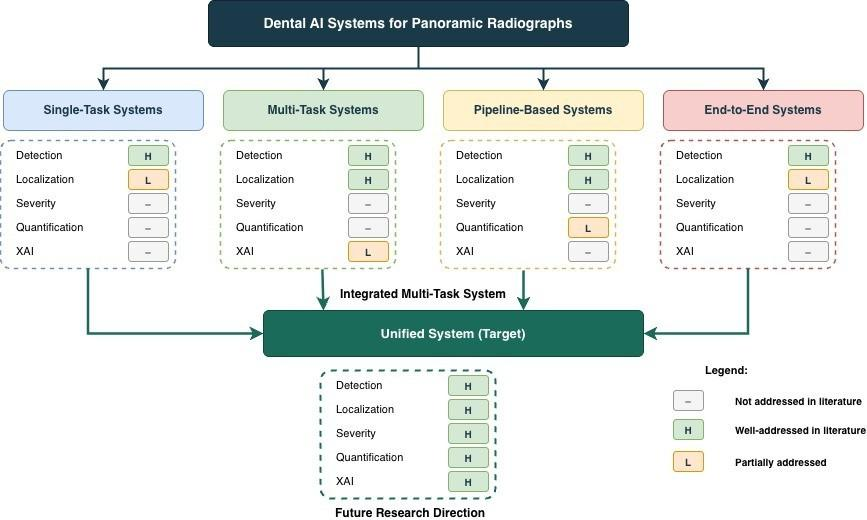
\includegraphics[width=0.8\textwidth]{figures/phase2/p2_3_02_taxonomy.jpg}
\caption[System-level taxonomy of dental AI approaches]{System-level taxonomy of dental AI approaches
for panoramic radiographs, adapted from the project's companion survey (Phase 2 report, Figure 3.2).}
\label{fig:taxonomy}
\end{figure}
